En este capítulo se exhibirán y discutiran los resultados obtenidos a lo largo del trabajo. Está dividido en dos secciones, la primera muetra los resultados de recintos con una única puerta y la segunda los resultados para recintos con dos puertas sobre la misma pared.  

\section{Una puerta}

En esta sección se compararán los campos de presión y velocidad para recintos con puerta ancha (3,6~m) y angosta (1,2~m), también se hará una comparación de la presión y velocidad en función del tiempo que soporta un individuo que comieza en el medio de la habitacón.    

\subsubsection{Puerta ancha (3,6~m)}

Los resultados que se muestran en esta subsección son de simulaciones hechas para un recinto de  $20\times 20$~(m) con 225 individuos y una puerta centrada en la posición $x=20$~m e $y=10$~m con un ancho $L=3,6$~m.\\
En la figura \ref{isobaras_3_6m} se muestra un gráfico de isobaras. Puede verse que la zona de mayor presión se da a los costados de la puerta mientras que en el medio la presión es menor (sobre todo en la zona más proxima a la puerta). La distribución de presiones es simétrica con respecto a la mitad del recinto en la coordenada y. 

\begin{figure}[H]
    \centering
    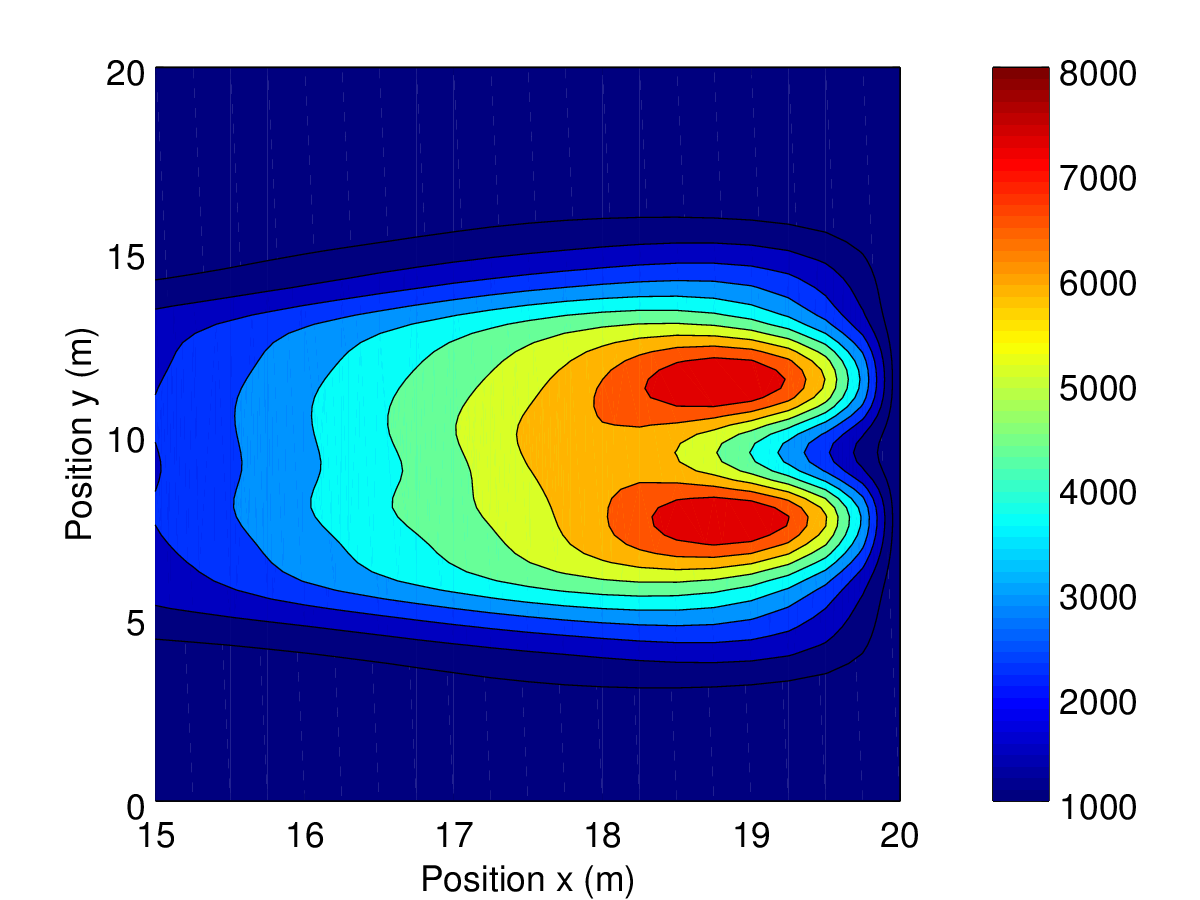
\includegraphics[height=5.5cm]{figuras/press_225p_v4_onedoor_3_6.png}
    \caption[width=5cm]{Isobaras cercanas a la puerta; la escala a la derecha está expresada en [PV]=N.m. La salida está centrada en la posición $x=20$~m e $y=10$~m y tiene ancho $L=3,6$~m. El recinto es de $20\times 20$~(m) con 225 individuos. La gráfica corresponde a valores medios a lo largo de 30 procesos de evacuación. Se usó un grillado de 1m$^2$ para promediar el campo de presiones (PV). La velocidad deseada de los individuos fue de $v_d=4$~m/s.}
    \label{isobaras_3_6m}
\end{figure}

El gráfico de la figura \ref{flujo_3_6} muestra el promedio del flujo de velocidades. El ancho del trazo denota la magnitud del módulo de la velocidad. La mayor celeridad se obtiene para la zona del medio (para la coordenada y), dando a entender que los individuos que se encuentran en en dicha región evacúan más rapido que los indvididuos que van por los costados. 
Puede verse que las zonas de alta presión coinciden con zonas de baja velocidad (costados) mientras que las zonas de alta velocidad son áreas con menor presión. 


\begin{figure}[H]
    \centering
    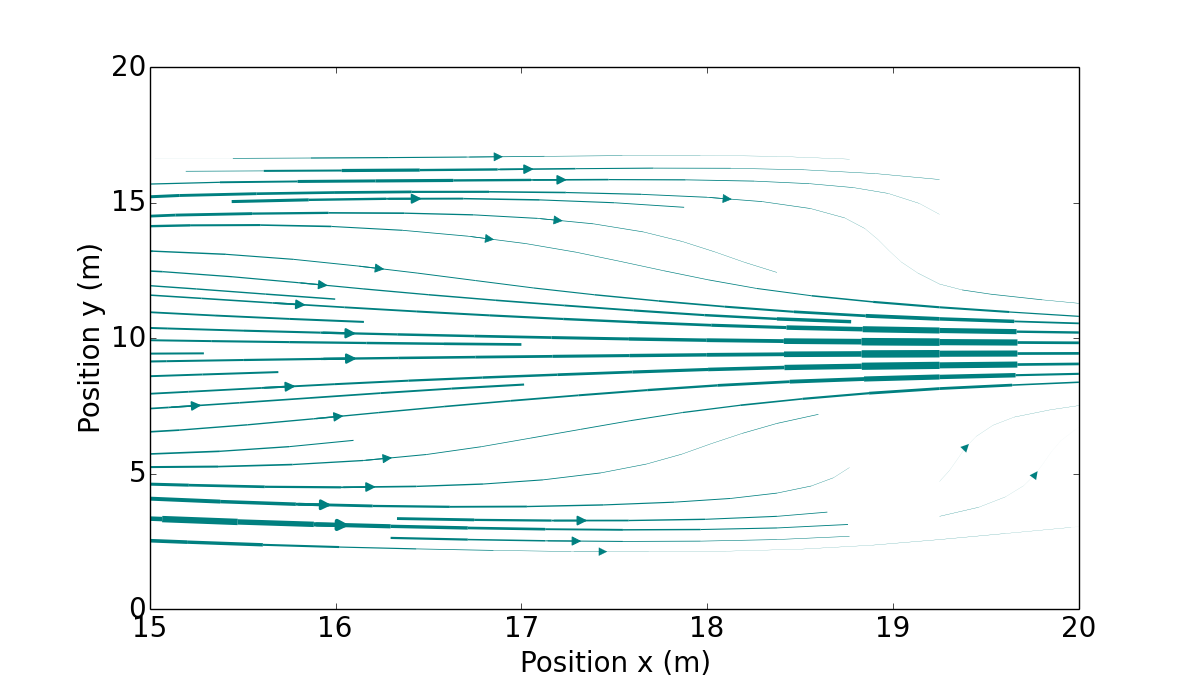
\includegraphics[height=5.5cm]{figuras/flujo_door_3_6m.png}
    \caption[width=5cm]{Gráfico de velocidad. La salida está centrada en la posición $x=20$~m e $y=10$~m y tiene ancho $L=3,6$~m. El recinto es de $20\times 20$~(m) con 225 individuos. La gráfica corresponde a valores medios a lo largo de 30 procesos de evacuación. Se usó un grillado de 1m$^2$ para promediar el campo de velocidades. La velocidad deseada de los individuos fue de $v_d=4$~m/s.}
    \label{flujo_3_6}
\end{figure}

La correlación espacial entre presión y velocidad se condice con los resultados obtenidos en la figura \ref{pv_vel_t_100_3_6}. Se muestra la presión y velocidad en función del tiempo para un individuo que comienza en el medio de la habitación ($x=20$~m e $y=10$~m). Al comienzo su velocidad aumenta sin que la presión se vea afectada ya que corre hacia la salida sin tocarse con el resto de los peatones. Luego, su velocidad disminuye y la presión que soporta aumenta. Este es el momento en el que la salida se obstruye y la multitud se amontona. Finalmente la velocidad vuelve a aumentar tanto como su presión disminuye, en este momento el individuo logra hacerse paso para evacuar. 

\begin{figure}[H]
    \centering
    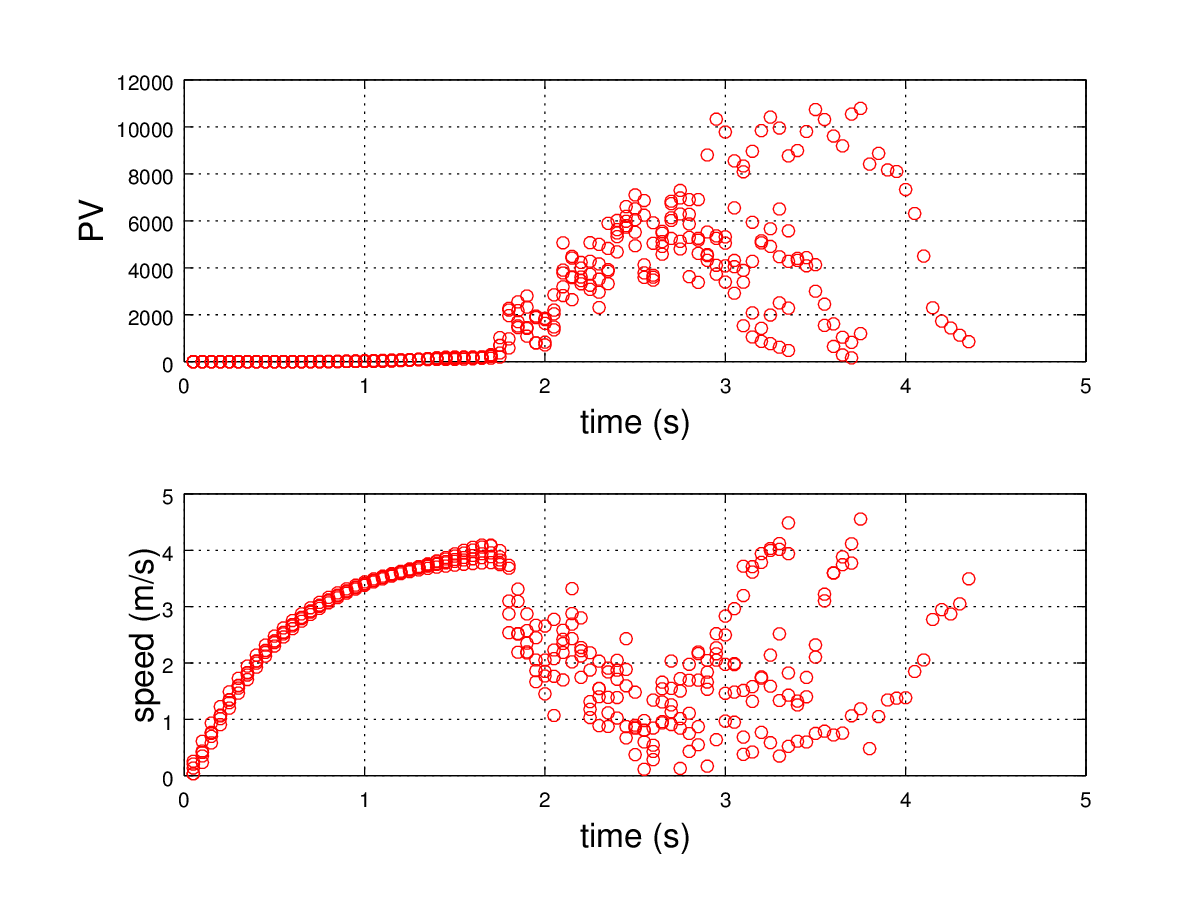
\includegraphics[height=5.5cm]{figuras/pv_vel_t_100_3_6.png}
    \caption[width=5cm]{Gráfico de velocidad(inferior) y presión(superior) en función del tiempo para un individuo ubicado inicialmente en $x=10$~m e $y=10$~m.  La salida está centrada en la posición $x=20$~m e $y=10$~m y tiene ancho $L=3,6$~m. El recinto es de $20\times 20$~(m) con 225 individuos. La gráfica corresponde a cinco iteraciones diferentes (variando la velocidad incial). La velocidad deseada del individuo fue de $v_d=4$~m/s.}
    \label{pv_vel_t_100_3_6}
\end{figure}

\subsubsection{Puerta angosta (1,2 m)}

Los resultados que se muestran en esta subsección son de simulaciones hechas para un recinto de  $20\times 20$~(m) con 225 individuos y una puerta centrada en la posición $x=20$~m e $y=10$~m con un ancho $L=1,2$~m.\\
En la figura \ref{isobaras_1_2m} se muestra la distribución de presión  para este tipo de recintos. Si bien se tiene una distribución simétrica, la presión maxima se da en el centro, a diferencia de lo que ocurre con recintos con puerta angosta donde la presión máxima está a los costados

\begin{figure}[H]
    \centering
    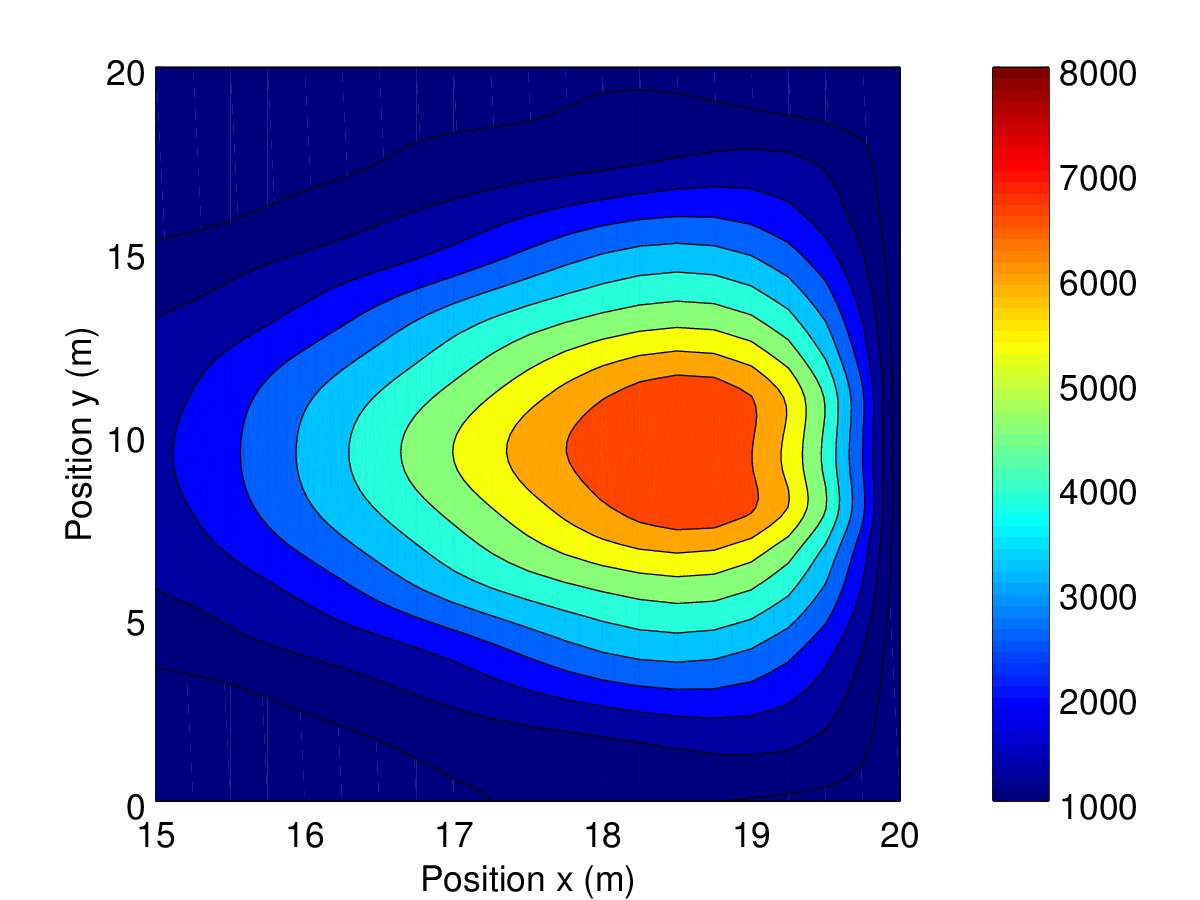
\includegraphics[height=5.5cm]{figuras/press_225p_v4_onedoor_1_2.png}
    \caption[width=5cm]{Isobaras cercanas a la puerta; la escala a la derecha está expresada en [PV]=N.m. La salida está centrada en la posición $x=20$~m e $y=10$~m y tiene ancho $L=1,2$~m. El recinto es de $20\times 20$~(m) con 225 individuos. La gráfica corresponde a valores medios a lo largo de 30 procesos de evacuación. Se usó un grillado de 1m$^2$ para promediar el campo de presiones (PV). La velocidad deseada de los individuos fue de $v_d=4$~m/s.}
    \label{isobaras_1_2m}
\end{figure}

En el gráfico de la figura \ref{flujo_1_2} se exhibe el flujo de velocidad. Al igual que en \ref{flujo_3_6}, la máxima celeridad se tiene en el medio (coordenada y).
Es notable que a diferencia de recintos con puerta ancha, la zona de mayor velocidad no coincida con una región de baja presión. De hecho se tiene máxima presión y velocidad en la misma área.  

\begin{figure}[H]
    \centering
    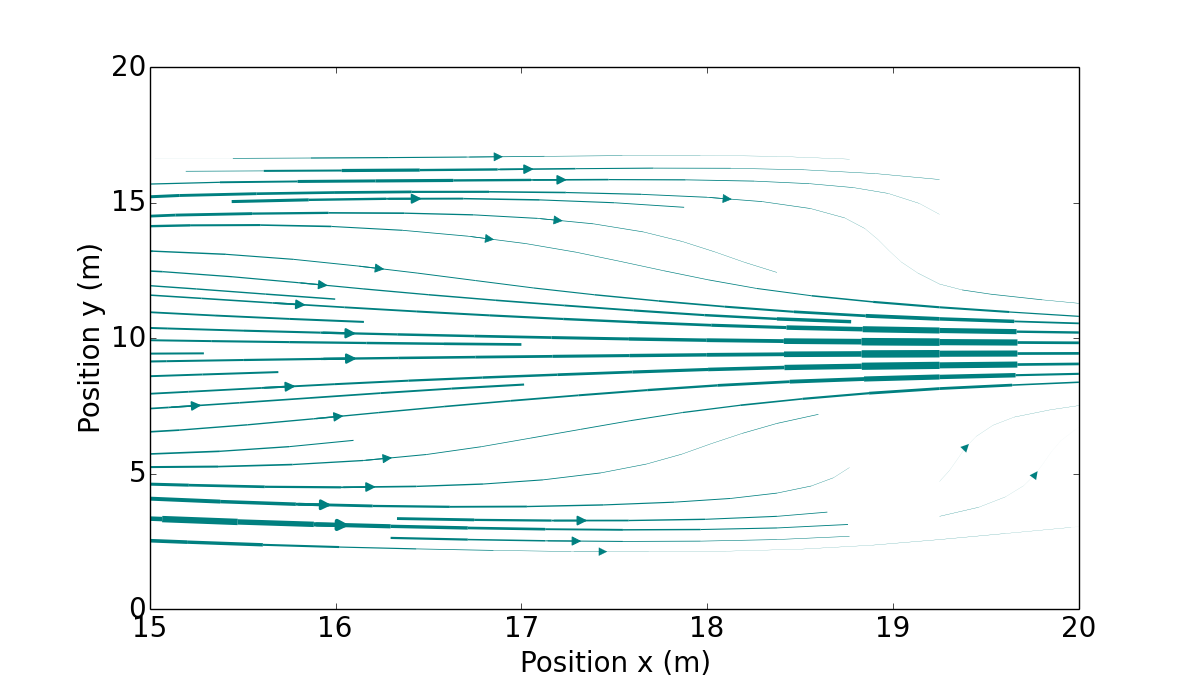
\includegraphics[height=5.5cm]{figuras/flujo_door_1_2m.png}
    \caption[width=5cm]{Gráfico de velocidad. La salida está centrada en la posición $x=20$~m e $y=10$~m y tiene ancho $L=1,2$~m. El recinto es de $20\times 20$~(m) con 225 individuos. La gráfica corresponde a valores medios a lo largo de 30 procesos de evacuación. Se usó un grillado de 1m$^2$ para promediar el campo de velocidades. La velocidad deseada de los individuos fue de $v_d=4$~m/s.}
    \label{flujo_1_2}
\end{figure}

En la figura \ref{pv_vel_t_100_1_2} se ve la correlación presión-velocidad que siente un individuo que comienza en el centro del recinto ($x=20$~m e $y=10$~m). Luego del estados estacionario (primeros segundos), los instantes en los que soporta alta presión, tiene baja velocidad y visceversa. Esto coincide con lo obtenido para un peatón ubicado con la misma posición inicial para una habitación con puerta angosta (fig. \ref{pv_vel_t_100_1_2}). \\
Puede decirse que la correlación presión-velocidad se pierde para el caso de recintos con puerta de $1,2$~m (en promedio espacial), sin embargo, para cada individuo en cada instante de tiempo, la correlación se mantiene. \\
La relación presión-velocidad presenta diferencias entre recintos con puerta ancha y puerta angosta ; los primeros tienen correlación tanto a nivel espacial (figs \ref{isobaras_3_6m} ) como a nivel temporal (fig \ref{flujo_3_6}). Se obtuvo que zonas de alta presión concuerdan con zonas de baja velocidad. El mismo comportamiento ocurre en cada instante para cada individuo. 
En cambio, cuando la puerta es angosta la zona de mayor presión es también zona de mayor velocidad (para promedio espacial) pero en cada instante de tiempo y para cada individuo se tiene que al soportar altas presiones sus velocidades son bajas y visceversa. \\
Esta diferencia se debe al hecho que cuando la puerta es ancha el flujo de la evacuación es permanente. Se forma un canal en el medio por donde los individuos transitan de forma continua. Esto tiene como consecuencia que la mayor velocidad se de en el medio y estimula la acumulación de peatones en los costados (formando focos de alta presión). No hay diferencias en cuanto al comportamiento presión-velocidad que sufren los individuos en cada instante de tiempo.
En cambio, cuando se trabaja con recintos de puerta angosta se tiene un flujo intermitente de evacuados. Por momentos el movimiento fluye y por momentos se encuentra detenido. Este efecto de Stop-and-go [cita] es determinante a la hora de promediar presión y velocidad ya que los momentos en los cueles la evacuación fluye aportan mucha velocidad en le medio (fig. \ref{flujo_1_2}) y en los momentos en los que las personas están quietas se suma mucha presión en el centro (fig. \ref{isobaras_1_2m}) por ser la región de mayor amontonamiento. Es por eso que para cada instante se preserva la correlación presión-velocidad pero para promedios espaciales se rompe.

\begin{figure}[H]
    \centering
    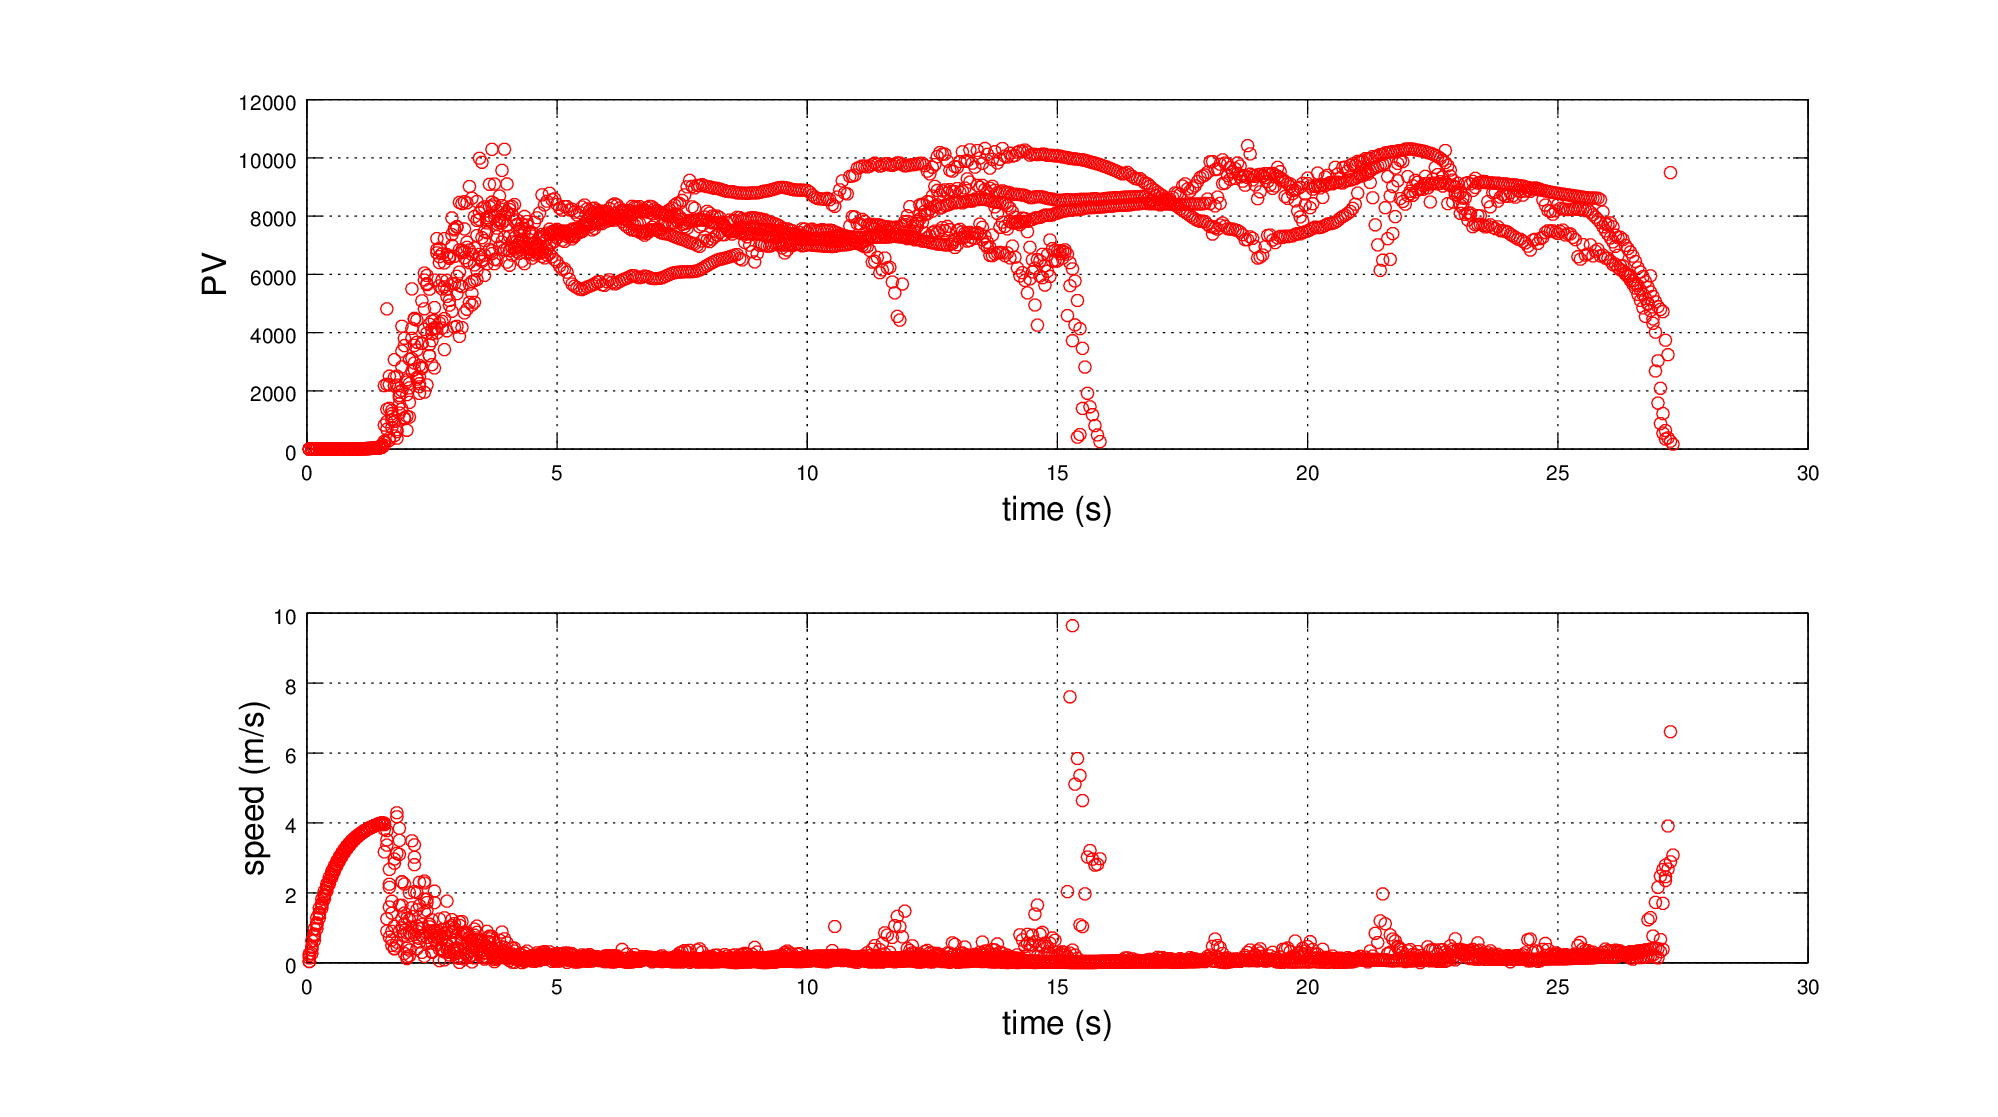
\includegraphics[height=5.5cm]{figuras/pv_vel_t_100_1_2.png}
    \caption[width=5cm]{Gráfico de velocidad(inferior) y presión(superior) en función del tiempo para un individuo ubicado inicialmente en $x=10$~m e $y=10$~m.  La salida está centrada en la posición $x=20$~m e $y=10$~m y tiene ancho $L=1,2$~m. El recinto es de $20\times 20$~(m) con 225 individuos. La gráfica corresponde a cinco iteraciones diferentes (variando la velocidad incial). La velocidad deseada del individuo fue de $v_d=4$~m/s.}
    \label{pv_vel_t_100_1_2}
\end{figure}


En está subsección se comparó la presión y velocidad tanto a nivel macroscópico (promedio espacial) como a nivel microscopico (variación temporal para un individuo en particular) para recintos con puerta angosta ($1,2$~m) y ancha ($3,6$~m). Se obtuvo que con puertas angostas surge el efecto Stop-and-go que provoca altas presiones en el centro mientras que con puertas anchas este efecto no aparece y la evacuación fluye permanentemente, con lo cual la mayor presión se da en los bordes de la puerta. La mayor velocidad se tiene en el medio para ambos recintos. Por lo tanto, la correlación presión-velocidad se verifica en habitaciones con puertas anchas (tanto a nivel macroscópico como a nivel microscópico) mientras que en recintos con puertas angostas solo se da a nivel microscópico.  


\section{Dos puertas}

En esta sección se muestran los resultados para recintos con dos puertas ubicadas sobre la misma pared. Se estudió como varía el tiempo de evacuación, la probabilidad de formar clusters de bloqueo y la distribución de presión como función del gap (distancia de separación entre puertas).  

\subsection{Faster is slower}


\subsection{Tiempo de evacuación}

En esta subsección se muestran los resultados de las mediciones de tiempo de evacuación en función de gap.
El tiempo de evacuación se define como el lapso que tarda una determinada cantidad de individuos $>70%$ en evacuar el recinto. 


\begin{figure}[H]
    \centering
    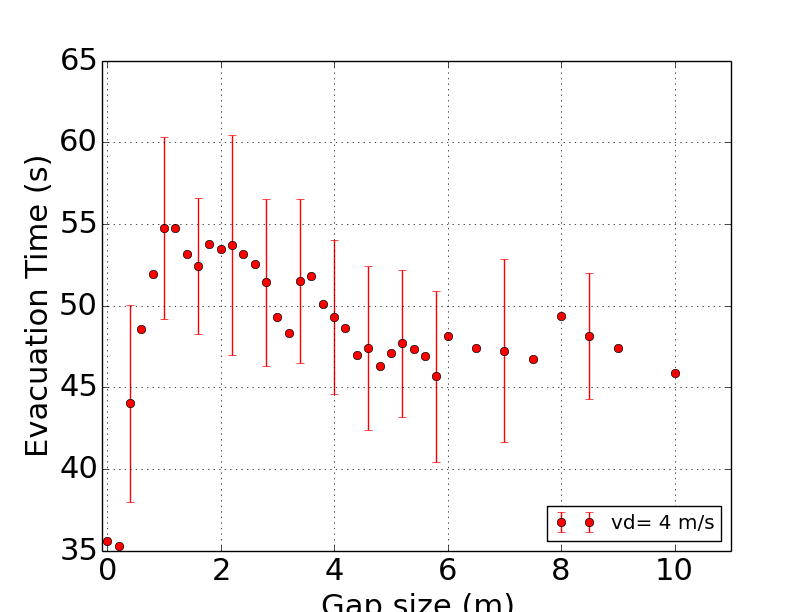
\includegraphics[height=5.5cm]{figuras/gap_vste_225p.png}
    \caption[width=5cm]{Gráfico de tiempo de evacuación en función del gap. El recinto es de $20\times 20$~(m) con 225 individuos y dos puertas, cada una tiene un ancho de $L=1,2$~m. La gráfica corresponde al promedio de treinta iteraciones. La velocidad deseada del individuo fue de $v_d=4$~m/s. Cada simulación termina cuando evacúan 160 individuos.}
    \label{sintesis}
\end{figure}

\begin{figure}[H]
    \centering
    \includegraphics[height=5.5cm]{figuras/gap_vsten.png}
    \caption[width=5cm]{Gráfico de tiempo de evacuación en función del gap para recintos de $20\times 20$~(m), $30\times 30$~(m) y $40\times 40$~(m) con 225, 580 y 961 individuos respectivamente. Todos los recintos tienen dos puertas, cada una de ancho $L=1,2$~m. Las gráficas corresponden al promedio de treinta iteraciones. Para todos los casos, la velocidad deseada del individuo fue de $v_d=4$~m/s. Cada simulación termina cuando evacúan 160, 529 y 961 individuos respectivamente.}
    \label{sintesis}
\end{figure}

\begin{figure}[H]
    \centering
    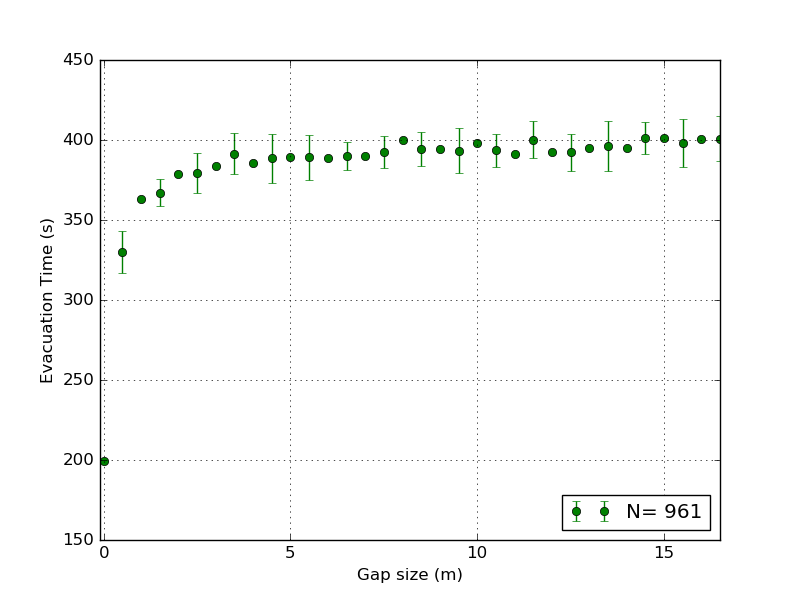
\includegraphics[height=5.5cm]{figuras/gap_vste_v4_961p.png}
    \caption[width=5cm]{Gráfico de tiempo de evacuación en función del gap. El recinto es de $40\times 40$~(m) con 961 individuos y dos puertas, cada una tiene un ancho de $L=1,2$~m. La gráfica corresponde al promedio de treinta iteraciones. La velocidad deseada del individuo fue de $v_d=4$~m/s. Cada simulación termina cuando evacúan 864 individuos.}
    \label{sintesis}
\end{figure}

\begin{figure}[H]
    \centering
    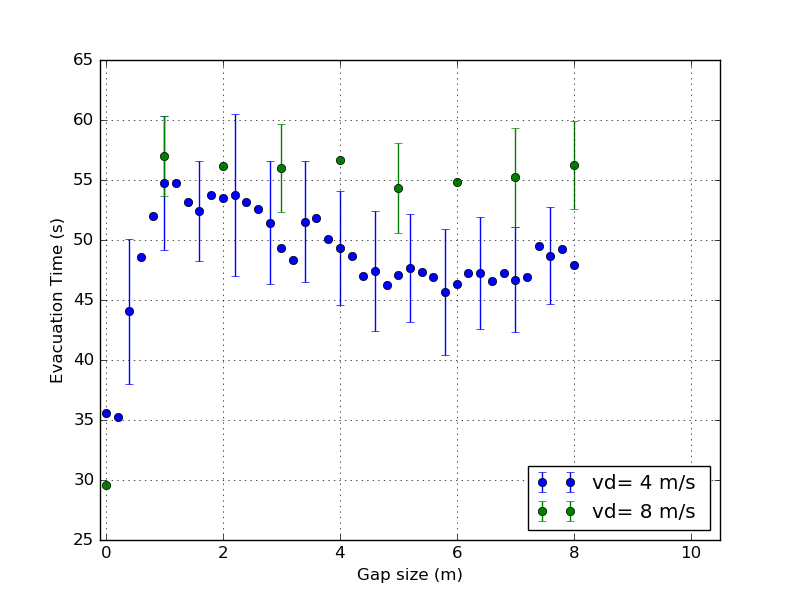
\includegraphics[height=5.5cm]{figuras/gap_vste_v4_v8.png}
    \caption[width=5cm]{Gráfico de tiempo de evacuación en función del gap. El recinto es de $20\times 20$~(m) con 225 individuos y dos puertas, cada una tiene un ancho de $L=1,2$~m. La gráfica corresponde al promedio de treinta iteraciones. Las velocidades de deseo de los individuos es de $v_d=4$~m/s y $v_d=8$~m/s. Cada simulación termina cuando evacúan 160 individuos.}
    \label{sintesis}
\end{figure}


\subsection{Blocking clusters}

\begin{figure}[H]
    \centering
    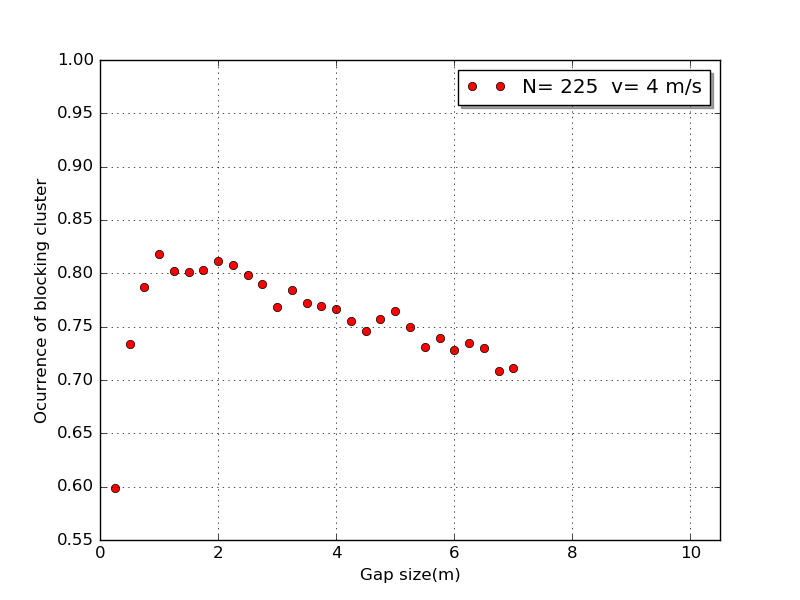
\includegraphics[height=5.5cm]{figuras/proba_vsgap_small_225p_v4.png}
    \caption[width=5cm]{Probabilidad de formar small blocking clusters (bloqueos de una sola puerta) en función del gap. El recinto es de $20\times 20$~(m) con 225 individuos y dos puertas, cada una tiene un ancho de $L=1,2$~m. La gráfica corresponde al promedio de treinta iteraciones. La velocidad de deseo es de $v_d=4$~m/s. Cada simulación termina cuando evacúan 160 individuos.}
    \label{sintesis}
\end{figure}

\begin{figure}[H]
    \centering
    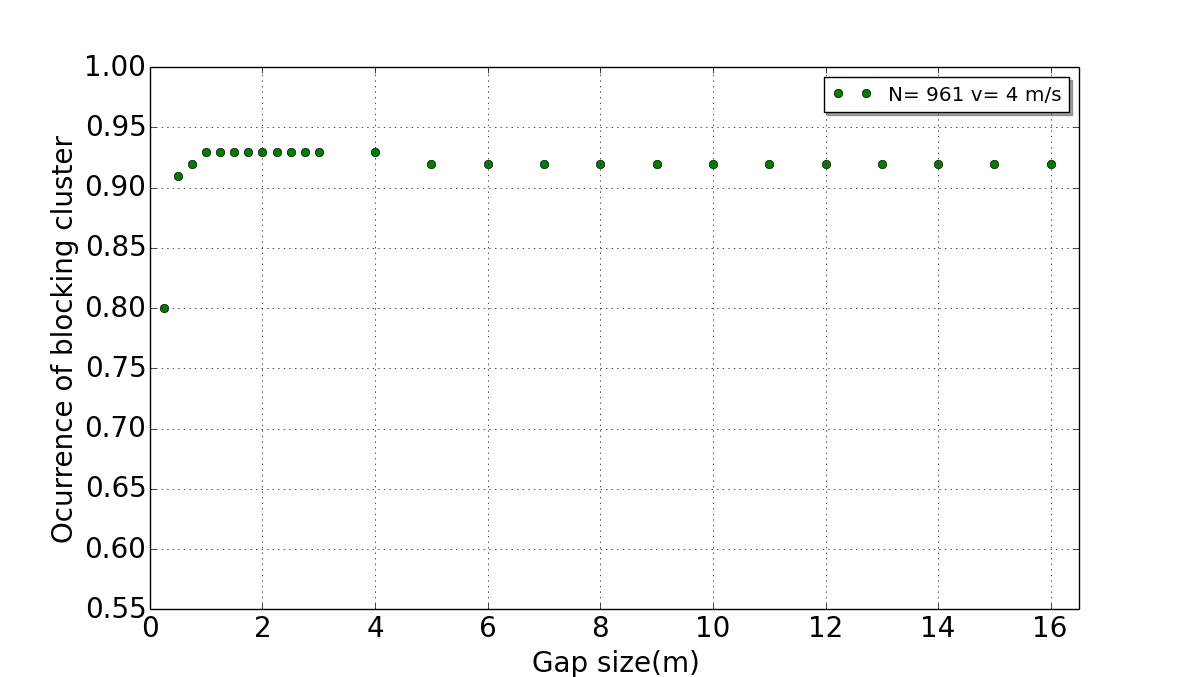
\includegraphics[height=5.5cm]{figuras/proba_vsgap_small_961p_v4.png}
    \caption[width=5cm]{Probabilidad de formar small blocking clusters (bloqueos de una sola puerta) en función del gap. El recinto es de $40\times 40$~(m) con 961 individuos y dos puertas, cada una tiene un ancho de $L=1,2$~m. La gráfica corresponde al promedio de treinta iteraciones diferentes. La velocidad de deseo es de $v_d=4$~m/s. Cada simulación termina cuando evacúan 864 individuos.}
    \label{sintesis}
\end{figure}

\begin{figure}[H]
    \centering
    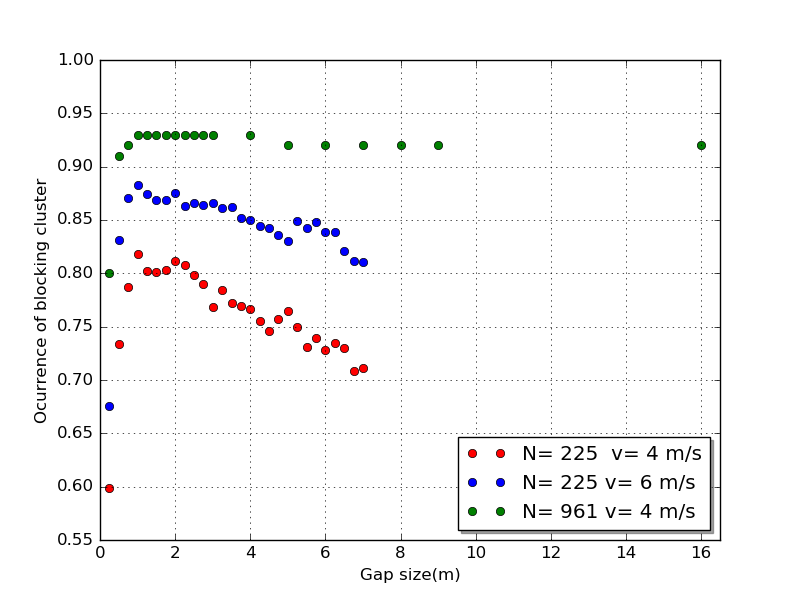
\includegraphics[height=5.5cm]{figuras/proba_vsgap_small_all.png}
    \caption[width=5cm]{Probabilidad de formar small blocking clusters (bloqueos de una sola puerta) en función del gap, para un recinto $20\times 20$~(m) con 225 individuos a $v_d=4$~m/s y $v_d=6$~m/s. Lo mismo para un recinto de $40\times 40$~(m) con 961 individuos a $v_d=4$~m/s. Ambos recintos poseén dos puertas, cada una tiene un ancho de $L=1,2$~m. Las gráficas corresponden al promedio de treinta iteraciones diferentes. Las simulación terminan cuando evacúan 160 individuos y 864 respectivamente.}
    \label{sintesis}
\end{figure}

\begin{figure}[H]
    \centering
    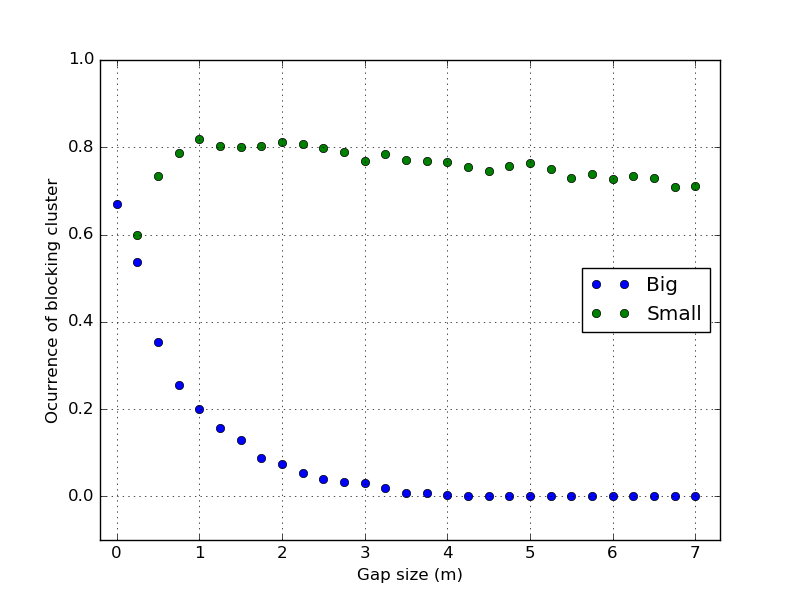
\includegraphics[height=5.5cm]{figuras/proba_vsgap_v4_big_small.png}
    \caption[width=5cm]{Probabilidad de formar big y small blocking clusters (bloqueos de dos y una puerta respectivamente) en función del gap. El recinto es de $20\times 20$~(m) con 225 individuos y dos puertas, cada una tiene un ancho de $L=1,2$~m. Las gráficas corresponden al promedio de treinta iteraciones diferentes. La velocidad de deseo es de $v_d=4$~m/s. Cada simulación termina cuando evacúan 160 individuos.}
    \label{sintesis}
\end{figure}



\subsection{Presión}

\begin{figure}[H]
    \centering
    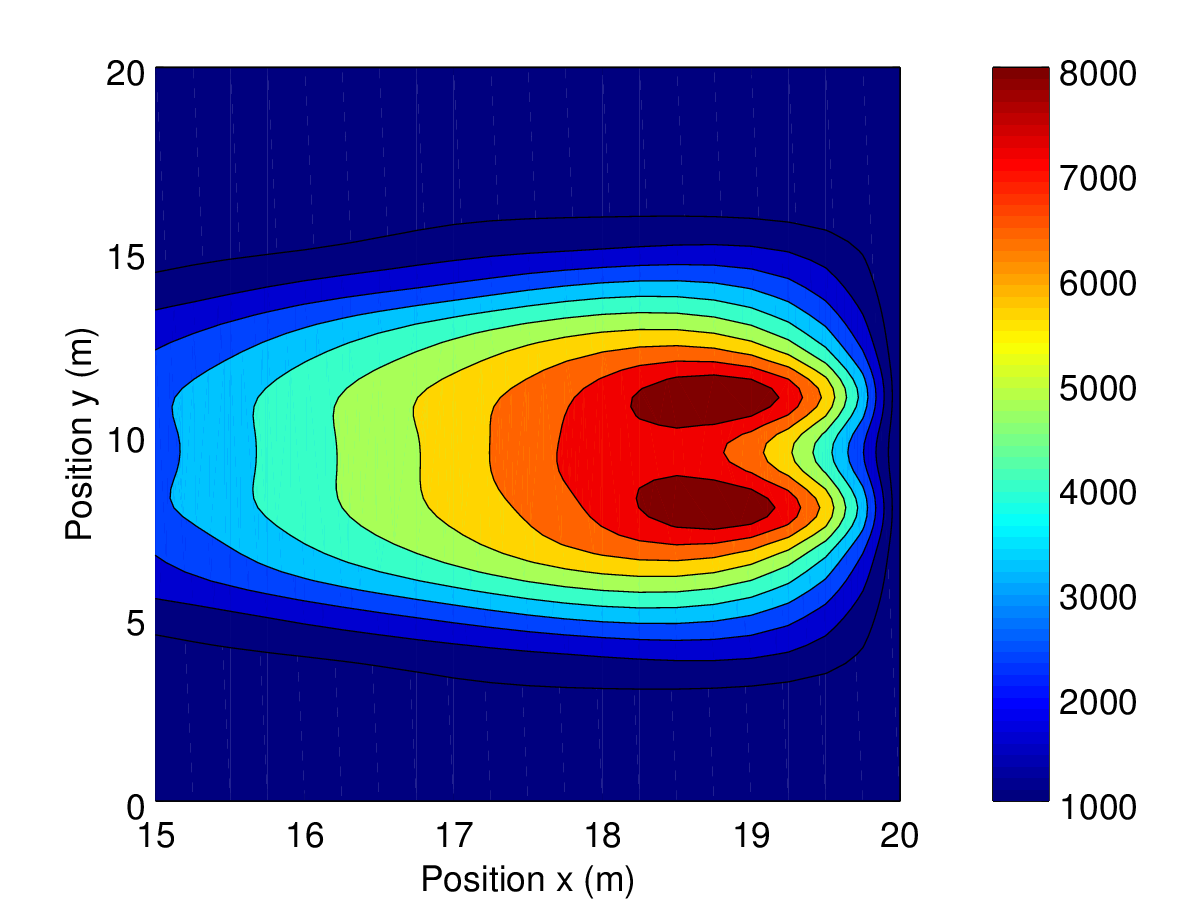
\includegraphics[height=5.5cm]{figuras/press_225p_v4_g0.png}
    \caption[width=5cm]{Isobaras cercanas a la puerta; la escala a la derecha está expresada en [PV]=N.m. La salida está centrada en la posición $x=20$~m e $y=10$~m, son dos puertas de ancho $L=1,2$~m con $g=0$~m. El recinto es de $20\times 20$~(m) con 225 individuos. La gráfica corresponde a valores medios a lo largo de 30 procesos de evacuación. Se usó un grillado de 1m$^2$ para promediar el campo de presiones (PV). La velocidad deseada de los individuos fue de $v_d=4$~m/s.}
    \label{presion_225p_g0}
\end{figure}

\begin{figure}[H]
    \centering
    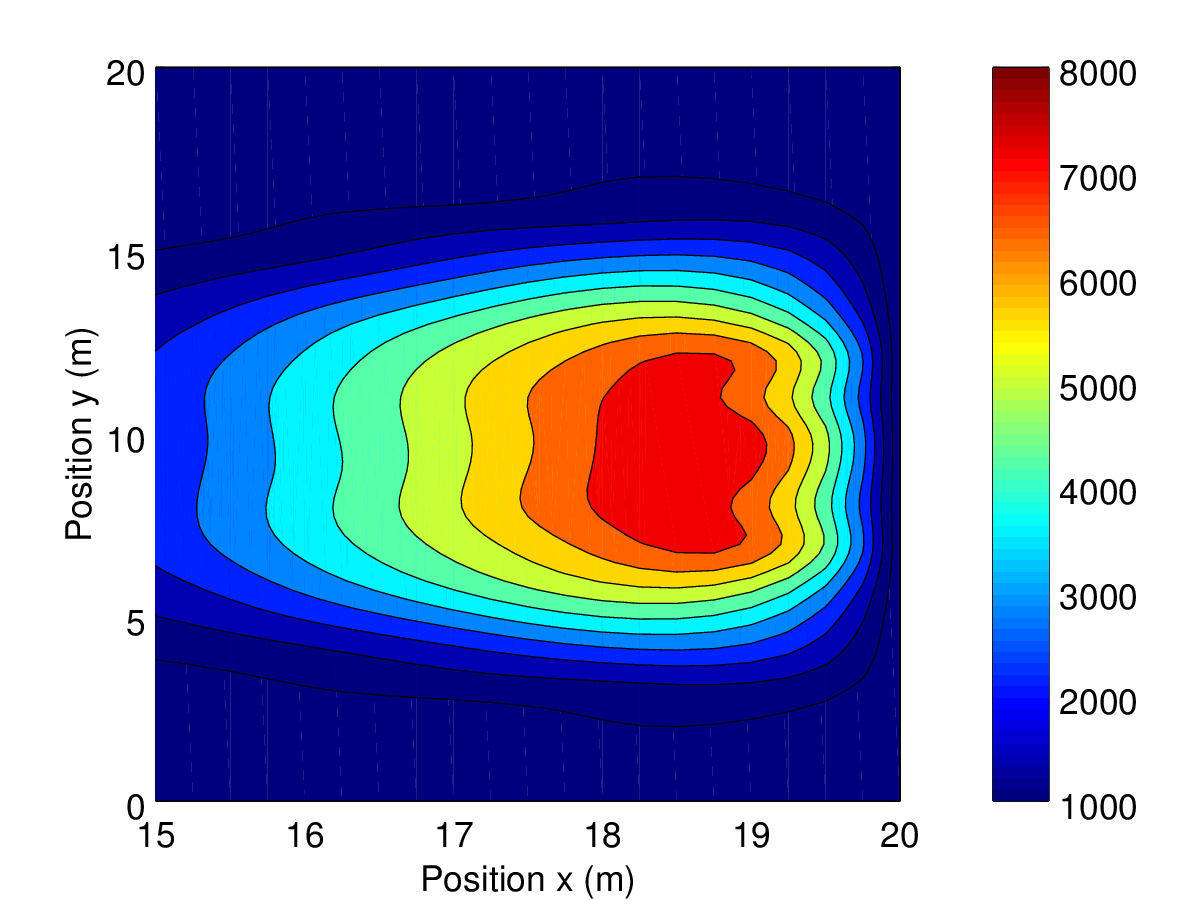
\includegraphics[height=5.5cm]{figuras/press_225p_v4_g1_5.png}
    \caption[width=5cm]{Isobaras cercanas a la puerta; la escala a la derecha está expresada en [PV]=N.m. La salida consta de dos puertas de ancho $L=1,2$~m separadas entre si por una distancia de $g=1,5$~m, centrdas en $x=20$~m e $y=11,35$~m y $x=20$~m e $y=8,65$~m . El recinto es de $20\times 20$~(m) con 225 individuos. La gráfica corresponde a valores medios a lo largo de 30 procesos de evacuación. Se usó un grillado de 1m$^2$ para promediar el campo de presiones (PV). La velocidad deseada de los individuos fue de $v_d=4$~m/s.}
    \label{presion_225p_g1_5}
\end{figure}

\begin{figure}[H]
    \centering
    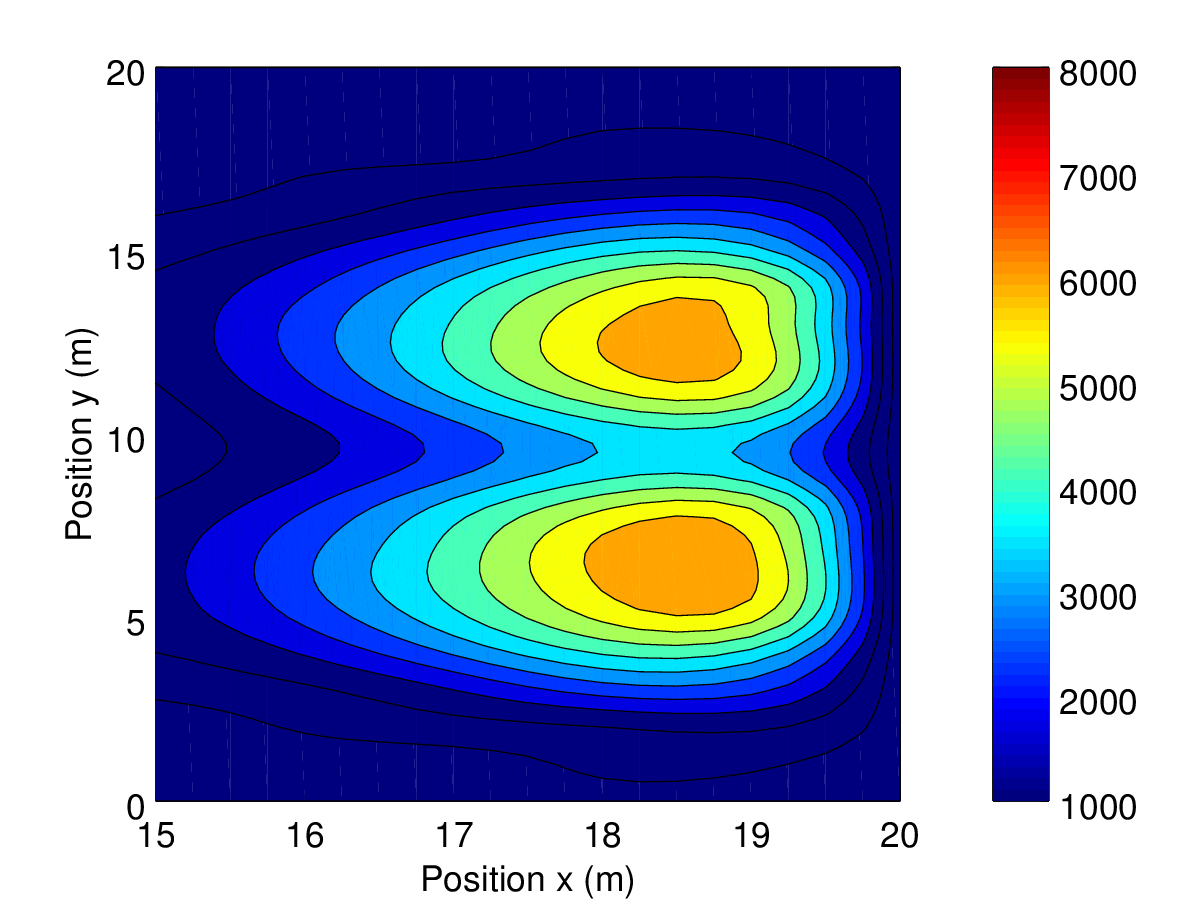
\includegraphics[height=5.5cm]{figuras/press_225p_v4_g5.png}			\caption[width=5cm]{Isobaras cercanas a la puerta; la escala a la derecha está expresada en [PV]=N.m. La salida consta de dos puertas de ancho $L=1,2$~m separadas entre si por una distancia de $g=1,5$~m, centrdas en $x=20$~m e $y=12,5$~m y $x=20$~m e $y=7,5$~m. El recinto es de $20\times 20$~(m) con 225 individuos. La gráfica corresponde a valores medios a lo largo de 30 procesos de evacuación. Se usó un grillado de 1m$^2$ para promediar el campo de presiones (PV). La velocidad deseada de los individuos fue de $v_d=4$~m/s.}
    \label{presion_225p_g5}
\end{figure}



\subsection{Comportamiento asintótico}


